The original 61 phonemes in the TIMIT corpus was mapped into 39 phonemes as suggested in {mapping}. This mapping is shown in table \ref{table:mapping}. The 39 phonemes are then used to both train and evaluate the model. 

\begin{table}[H]
\centering
    \begin{tabular}{ | l | l |}
    \hline
    aa, ao & aa \\ \hline
    ah, ax, ax-h  & ah \\ \hline
    er, axr & er \\ \hline
    hh, hv & hh \\ \hline   
    ih, ix & ih \\ \hline
	l, el & l \\ \hline
	m, em & m \\ \hline
	n, en, nx & n \\ \hline
	ng, eng & ng \\ \hline
	sh, zh & sh \\ \hline
	uw, ux & uw \\ \hline
	pcl, tcl, kcl, bcl, dcl, gcl, h\#, pau, epi & sil \\ \hline
	q & - \\ \hline
    \end{tabular}
    \caption{Mapping the 61 original TIMIT phonemes(left) into 39 phonemes(right) as suggested in \cite{mapping}}
    \label{table:mapping}
\end{table}


We have tried different networks with different data sets (train/validation split). As a proof of concept, we trained the network for only two phonemes. Figure~\ref{fig:twoClass} shows the graphs of training error and validation error as well as accuracy at each epoch for this network. Reaching 100\% accuracy after 5 epochs, suggested that our data representation, along with the chosen network architecture, was in deed capable of separating different classes. Figure~\ref{fig:best} shows a similar graph for our best performing method on all 39 classes.

Table~\ref{table:results} shows a detailed listing of the setup and performance of different experiments.

\begin{table}
\hskip-2.7cm\begin{tabular}{|c|c|c|c|c|c|c|}
\hline
Name & Val Split \% & Phone Count & Conv. Layers Setup & Fully Con. Setup & Accuracy & Epochs \\
\hline
EXP1 & 25 & 2 (dr1) & 96, 256, 384, 384, 256, 256 & 256, 128, 2 & 100\% & 30 \\
\hline
EXP2 & 25 & 61 (dr1,dr2) & 96, 256, 384, 384, 256, 256 & 256, 128, 61 & 60\% & 30 \\
\hline
EXP3 & 25 & 39 (all) & 96, 256, 384, 384, 256, 256 & 4096, 2048, 39 & 65\% & 50 \\
\hline
\end{tabular} 
\caption{\label{table:results} Details of different experiments. Columns from left to right: experiment code-name, percentage of validation split, number of phonemes used and the regions included, number of nodes in different Convolutional layers, number of nodes in Fully Connected layers, Validation Accuracy and number of Epochs of the training.}
\end{table}

\begin{table}
\centering
\begin{tabular}{|c|c|}
\hline
Experiment & Unseen Test Error\\
\hline
EXP2 & 81\% \\
EXP3 & 79\% \\
\hline
\end{tabular}
\caption{\label{table:unseen} Error results on unseen test dataset.}
\end{table}

\begin{figure}[H]
\centering
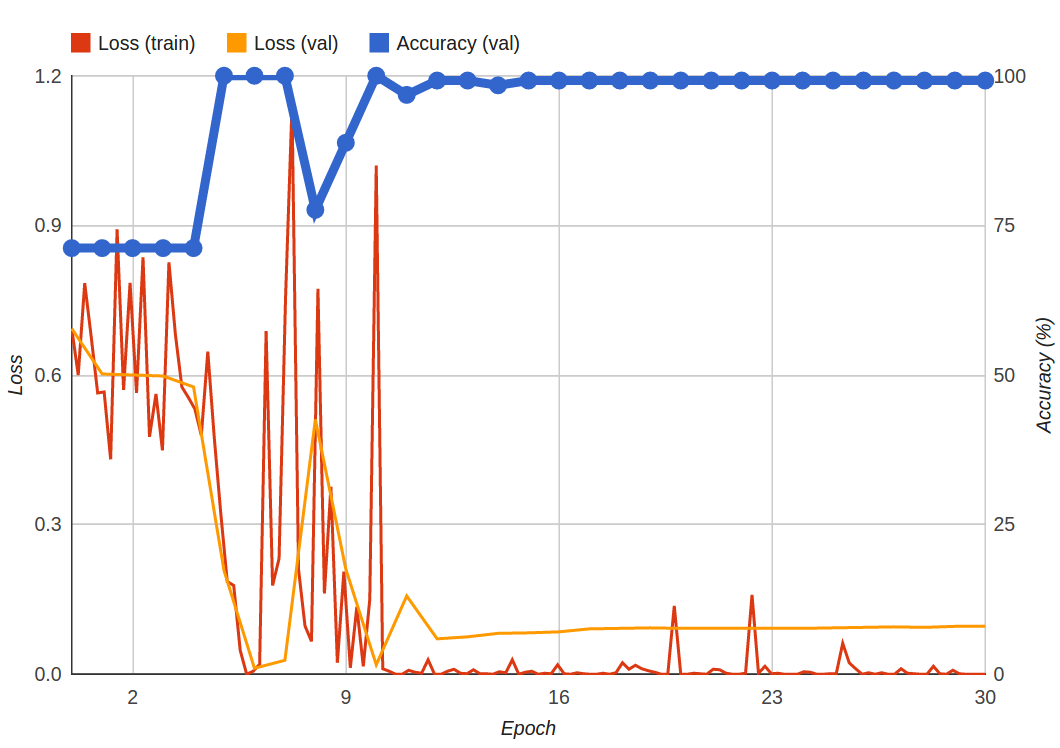
\includegraphics[scale=0.25]{figs/twoclass.png}
\caption{\label{fig:twoClass}Training error, Validation error and Accuracy for each epoch of training the AlexNet on two classes.}
\end{figure}

\begin{figure}[H]
\centering
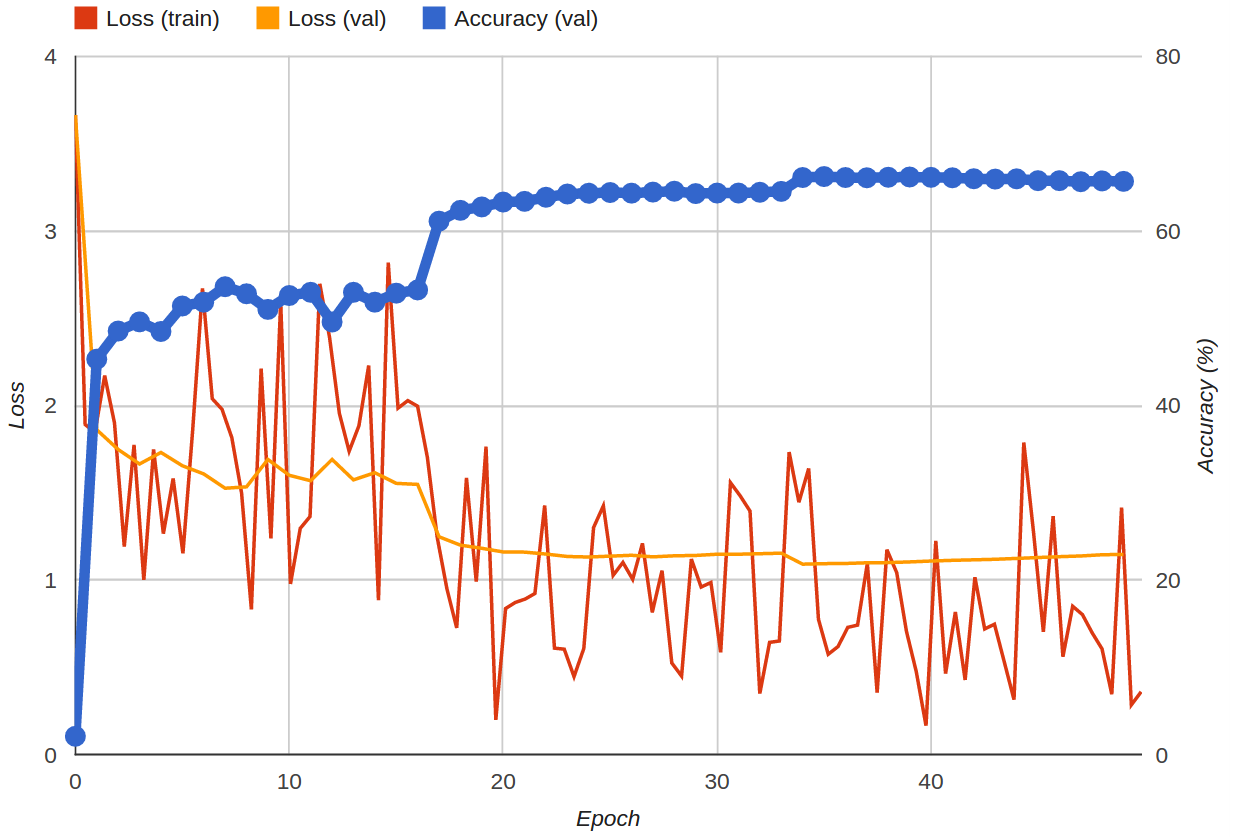
\includegraphics[scale=0.25]{figs/allclass.png}
\caption{\label{fig:best}Training error, Validation error and Accuracy for each epoch of training the best model on all 39 classes.}
\end{figure}




